\documentclass[]{article}
\usepackage{lmodern}
\usepackage{amssymb,amsmath}
\usepackage{ifxetex,ifluatex}
\usepackage{fixltx2e} % provides \textsubscript
\ifnum 0\ifxetex 1\fi\ifluatex 1\fi=0 % if pdftex
  \usepackage[T1]{fontenc}
  \usepackage[utf8]{inputenc}
\else % if luatex or xelatex
  \ifxetex
    \usepackage{mathspec}
  \else
    \usepackage{fontspec}
  \fi
  \defaultfontfeatures{Ligatures=TeX,Scale=MatchLowercase}
\fi
% use upquote if available, for straight quotes in verbatim environments
\IfFileExists{upquote.sty}{\usepackage{upquote}}{}
% use microtype if available
\IfFileExists{microtype.sty}{%
\usepackage{microtype}
\UseMicrotypeSet[protrusion]{basicmath} % disable protrusion for tt fonts
}{}
\usepackage[margin=1in]{geometry}
\usepackage{hyperref}
\hypersetup{unicode=true,
            pdftitle={Nutrition Report 2017},
            pdfborder={0 0 0},
            breaklinks=true}
\urlstyle{same}  % don't use monospace font for urls
\usepackage{graphicx,grffile}
\makeatletter
\def\maxwidth{\ifdim\Gin@nat@width>\linewidth\linewidth\else\Gin@nat@width\fi}
\def\maxheight{\ifdim\Gin@nat@height>\textheight\textheight\else\Gin@nat@height\fi}
\makeatother
% Scale images if necessary, so that they will not overflow the page
% margins by default, and it is still possible to overwrite the defaults
% using explicit options in \includegraphics[width, height, ...]{}
\setkeys{Gin}{width=\maxwidth,height=\maxheight,keepaspectratio}
\IfFileExists{parskip.sty}{%
\usepackage{parskip}
}{% else
\setlength{\parindent}{0pt}
\setlength{\parskip}{6pt plus 2pt minus 1pt}
}
\setlength{\emergencystretch}{3em}  % prevent overfull lines
\providecommand{\tightlist}{%
  \setlength{\itemsep}{0pt}\setlength{\parskip}{0pt}}
\setcounter{secnumdepth}{0}
% Redefines (sub)paragraphs to behave more like sections
\ifx\paragraph\undefined\else
\let\oldparagraph\paragraph
\renewcommand{\paragraph}[1]{\oldparagraph{#1}\mbox{}}
\fi
\ifx\subparagraph\undefined\else
\let\oldsubparagraph\subparagraph
\renewcommand{\subparagraph}[1]{\oldsubparagraph{#1}\mbox{}}
\fi

%%% Use protect on footnotes to avoid problems with footnotes in titles
\let\rmarkdownfootnote\footnote%
\def\footnote{\protect\rmarkdownfootnote}

%%% Change title format to be more compact
\usepackage{titling}

% Create subtitle command for use in maketitle
\newcommand{\subtitle}[1]{
  \posttitle{
    \begin{center}\large#1\end{center}
    }
}

\setlength{\droptitle}{-2em}
  \title{Nutrition Report 2017}
  \pretitle{\vspace{\droptitle}\centering\huge}
  \posttitle{\par}
  \author{}
  \preauthor{}\postauthor{}
  \date{}
  \predate{}\postdate{}


\begin{document}
\maketitle

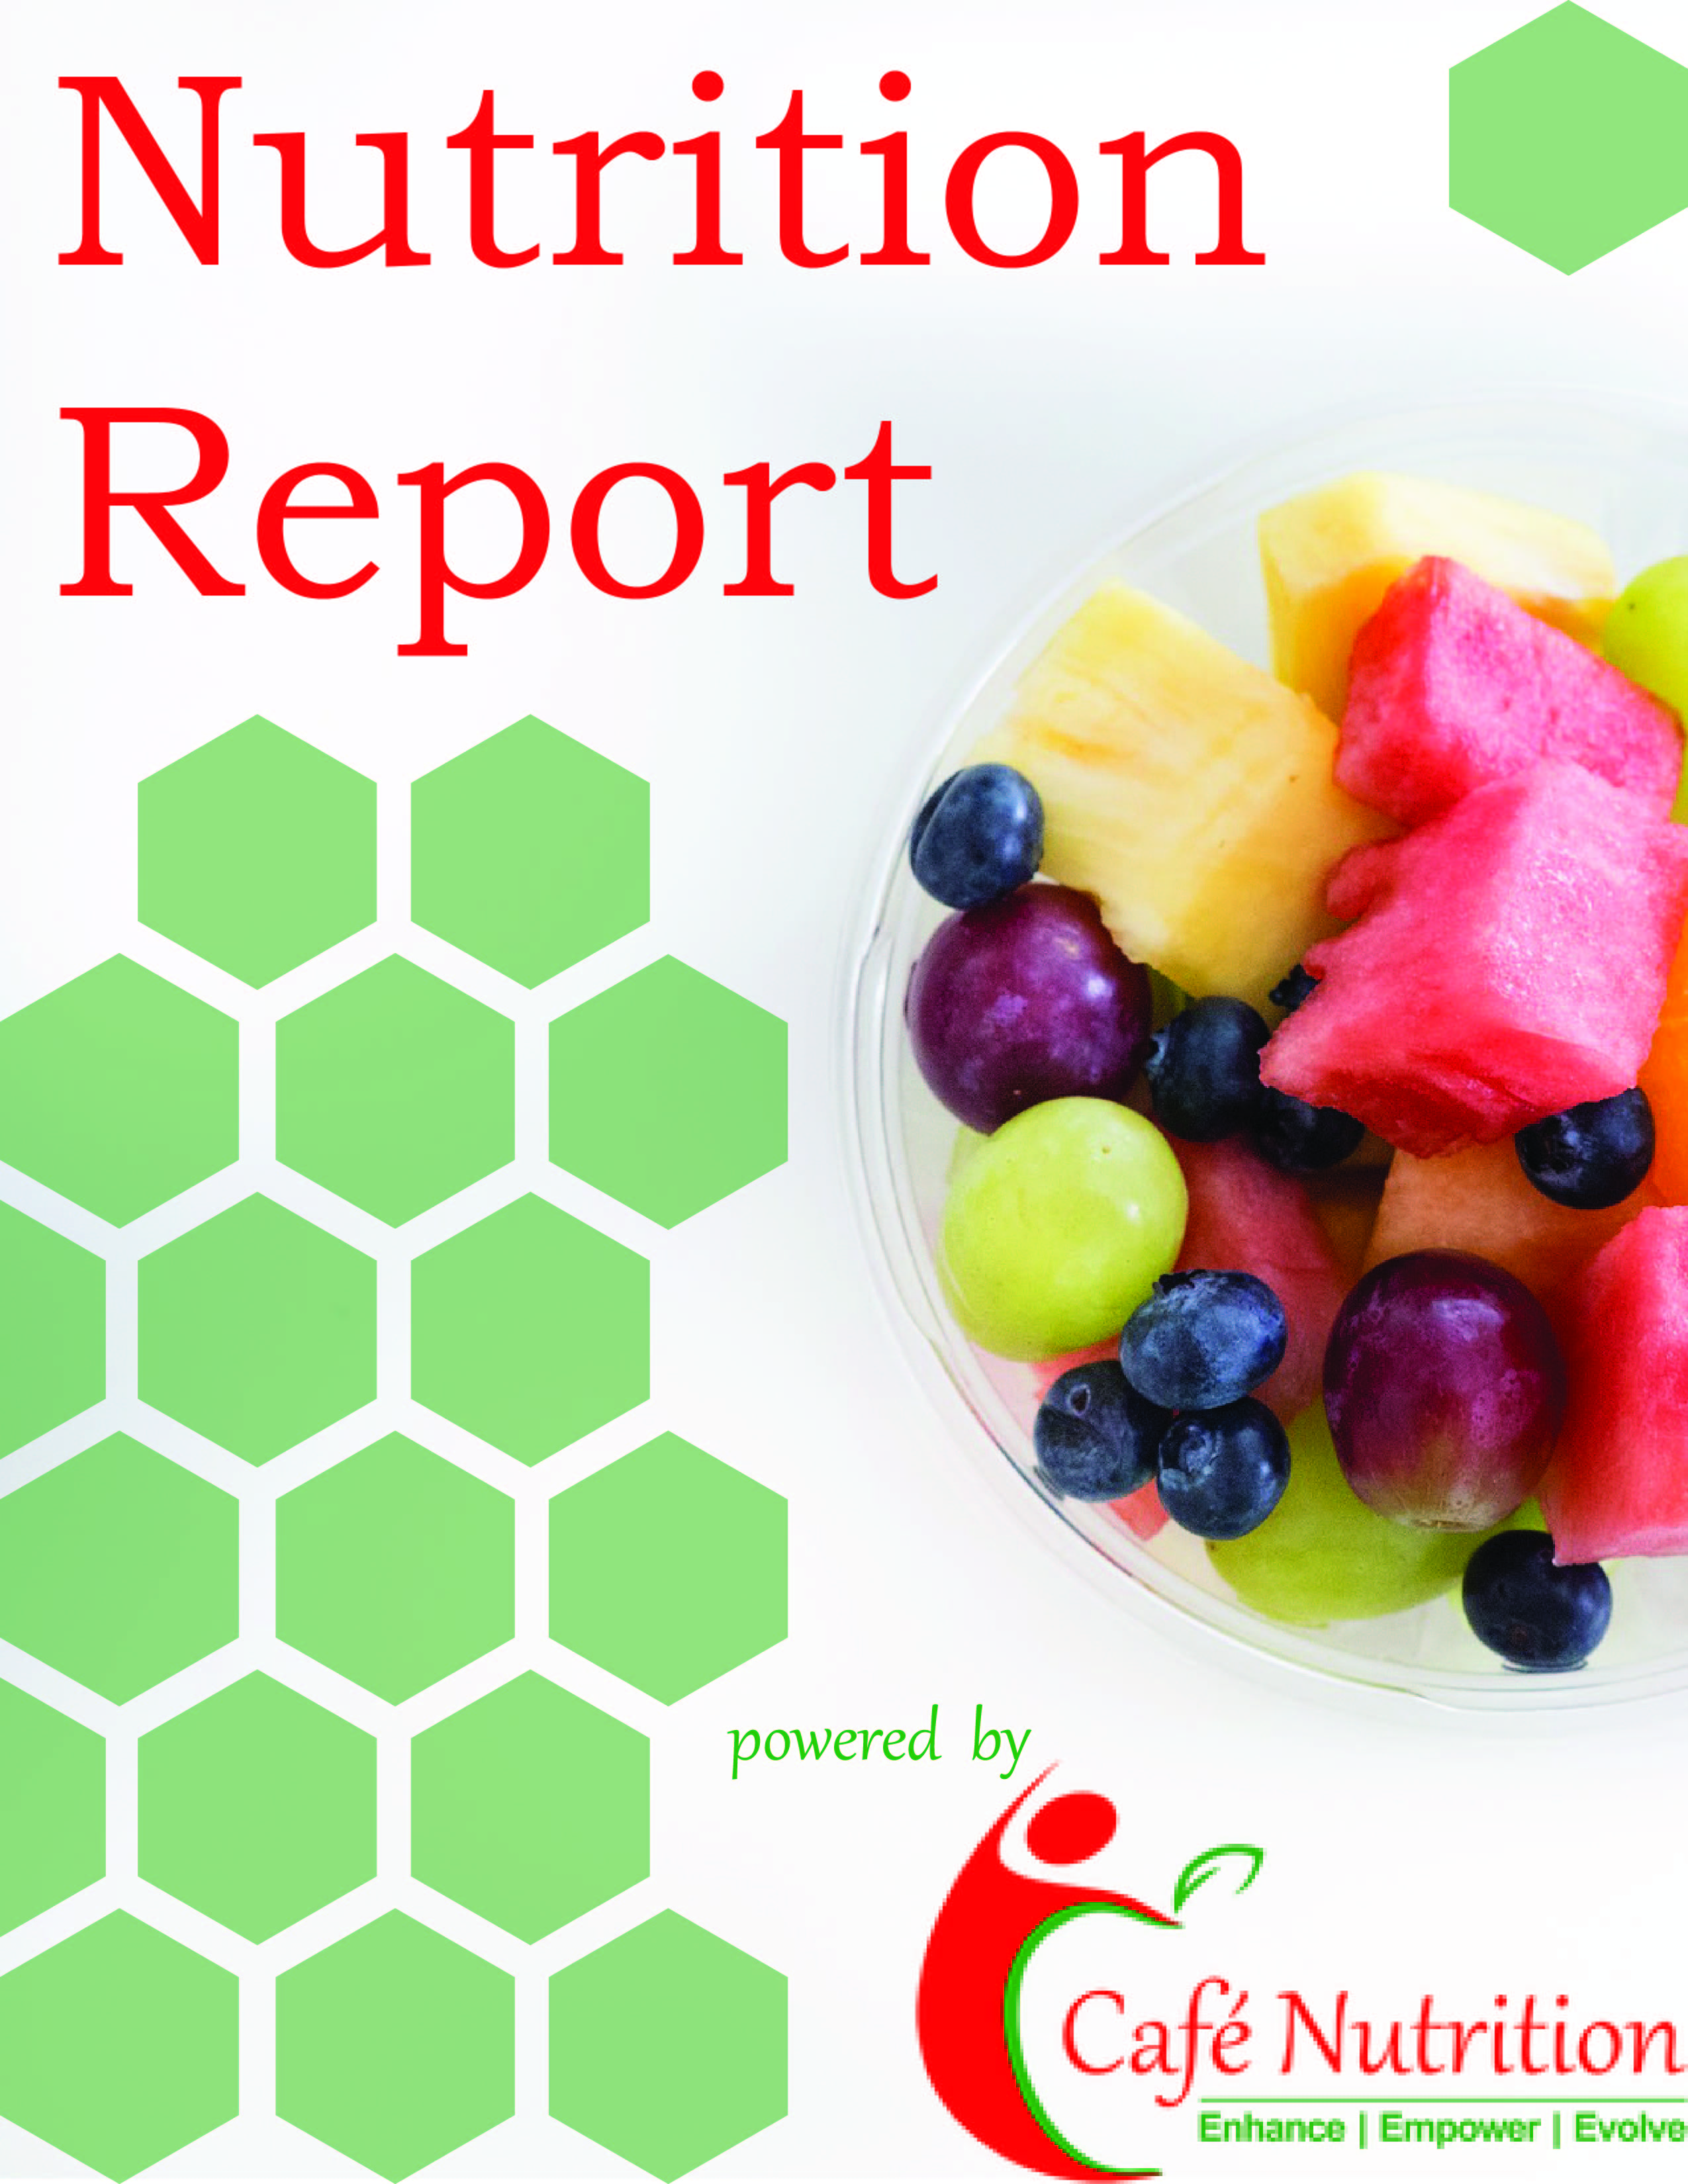
\includegraphics{../Files/title_page.jpg}

\newpage

\begin{center}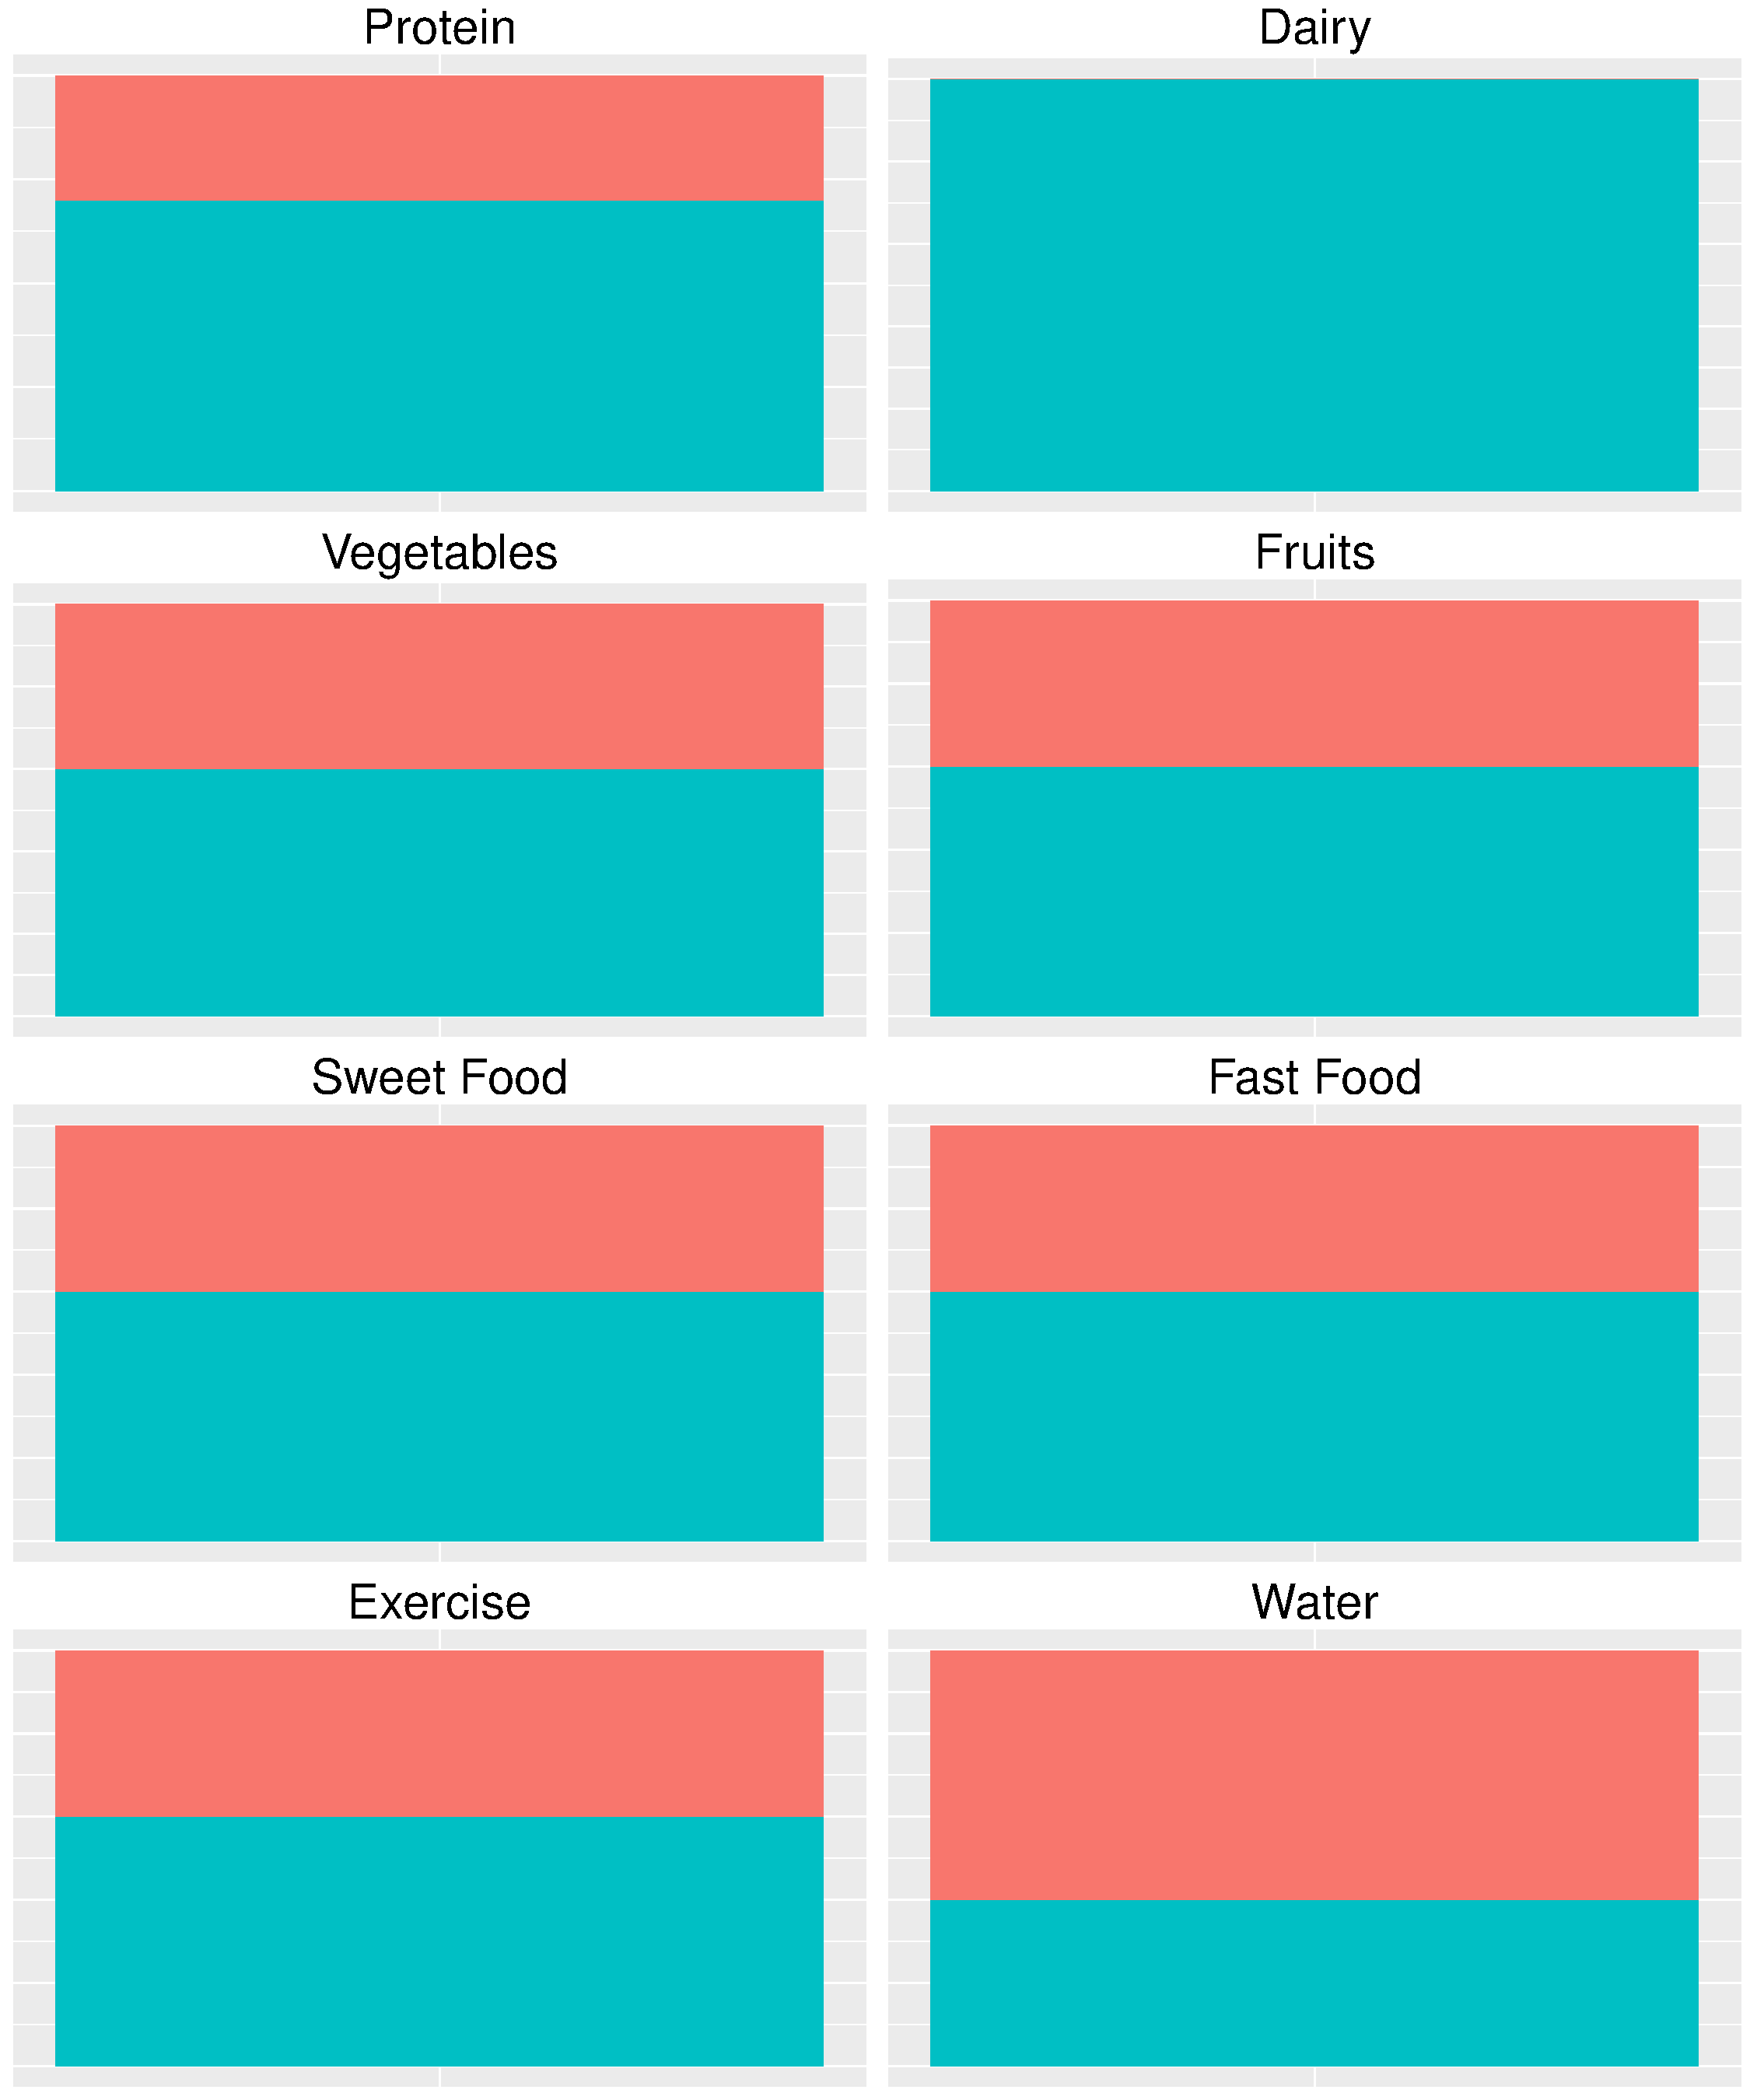
\includegraphics{Vrushti_Modi_report_files/figure-latex/unnamed-chunk-3-1} \end{center}

Your child Vrushti has a total nutrition score of 46 out of 50 possible
points. Read on to know what you're doing well and how you can get even
better

\begin{verbatim}
## [1] 4 4
\end{verbatim}

\begin{center}\includegraphics{Vrushti_Modi_report_files/figure-latex/unnamed-chunk-4-1} \end{center}

A higher proportion of blue green indicates better performance. For
example, blue/green in vegetables indicates that your child is getting
enough vegetables, while more blue/green in junk food and screen
indicates your child is getting \emph{less} junk and screen time

\newpage

\section{Things You're Doing Well}\label{things-youre-doing-well}

\subsection[Vegetables]{\texorpdfstring{Vegetables\protect
\includegraphics{../Files/vegetable.jpg}}{Vegetables}}\label{vegetables}

Good job! is getting share of vegetables. They have nutrients that can
boost immunity and keep ailments like a common cold and flu at bay. It's
especially important that Vrushti is eating vegetables at this early age
because food tastes are formed young. Eating vegetables in a rainbow of
colors will provide a wide range of nutrients that will help keep
Vrushti healthy

\subsection{\texorpdfstring{Fruits\emph{}}{Fruits}}\label{fruits}

is getting enough fruit. Fruits give you sustainable energy, unlike
sugar highs that last a few hours or less. Fruits also have many
micronutrients. For example, citrus fruits and strawberries are rich in
immune system-boosting vitamin C. Apples contain 16 different
polyphenols, which are antioxidants with health-promoting properties.
Eating fruits and vegetables in a rainbow of colors will provide a wide
range of nutrients that will help keep healthy

\subsection{Exercise}\label{exercise}

seems to be getting enough physical activity. This is especially
important at a young age because physical (body) and cognitive (brain)
development go hand-in-hand. While this continues for life, this
relationship is most critical at a young age. When kids are active,
their brain develops, allowing for new types of activity. Frequent
physical activity has been associated with improved behavior in the
classroom and beyond. Aerobic activity has been shown to increase the
size of essential brain structures and number of neural connections.

\subsection{Water}\label{water}

is getting enough water. Let this continue as kids don't always
recognise the early stages of thirst, which can make them particularly
vulnerable to becoming dehydrated, especially during times that can
drive up their body fluid losses, for example when they are playing
sport or during warm weather. Dehydration, even if only mild, can cause
tiredness, headaches, lack of concentration, reduced mental performance
and dry skin.

\newpage

\section{Things You Could Improve at}\label{things-you-could-improve-at}

Below are some tips on how you could improve Vrushti health and
nutrition. After going through the bulleted tips and your appointment
with the nutritionist, we reccomend you selct 3-5 tips to focus on and
improve over the next year

\subsection{Protein}\label{protein}

needs to get more protein. Protein repairs your builds and repairs body
tissue and organs, especially vital at this age. Proteins also form
antibodies that help prevent infection, illness, and disease. The
following foods contain

\begin{itemize}
\item
  Dals and beans
\item
  Nuts and seeds
\item
  Eggs and poultry
\item
  Fish
\end{itemize}

\subsection[Dairy]{\texorpdfstring{Dairy\protect
\includegraphics{../Files/dairy.jpg}}{Dairy}}\label{dairy}

could do with some more dairy. Dairy and dairy-containing foods
contribute many essential nutrients. Calcium and Vitamin D, especially,
are most easily absorbed from dairy.Both these nutrients are important
in ensuring that has healthy bones and teeth. You could squeeze in a
serving as a snack in the evening, or a cup of yogurt post the evening
play. Here are some other tips to increase dairy intake:

\begin{itemize}
\item
  Add milk in homemade puddings or fruit custards. You can control sugar
  with homemade stuff.
\item
  Parathas with paneer
\item
  Cheese cubes with fruit can be a great snack
\end{itemize}

\subsection[Junk Food]{\texorpdfstring{Junk
Food\protect
\includegraphics{../Files/sugar.png}}{Junk Food}}\label{junk-food}

could reduce consumption of sweet and/or fried food. Apart from
promoting obesity and cardiac disease, sugar can have a harmful effect
on academic performace. In an interesting study, researchers fed normal
preschoolers a high-sugar drink containing the amount of sugar in the
average can of soda and compared them with children who received a
non-sugar drink. The sugar group experienced decreased learning
performance and more hyperactivity than the non-sugar group. Here are
some strateges for how to do that

\begin{itemize}
\item
  Parents - lead by example. If children see you snacking on sweet foods
  and drinks they will follow you
\item
  Set a specific day and mealtime for dessert
\item
  Offer sweet fruits or dried fruits as snacks
\item
  Buy plain yogurt instead of the flavoured one and sweeten it with
  dried fruits or berries to enhance the taste
\item
  Stock your home with healthy snacking options like dried fruits, nuts,
  fruits and vegetables with dips like hummus and curd dips etc
\item
  Cook healthier alternatives of junk food eg baked fries instead of
  frying them, homemade pizzas with the healthy base and sauce, homemade
  burgers, whole wheat pastas, etc
\end{itemize}

\subsection{Screen Time}\label{screen-time}

It would be good for to spend less time on screens. Excessive screen
time at a young age can be harmful in many ways. For example, tablets
are the ultimate shortcut tools. Unlike a mother reading a story to a
child, for example, a smartphone-told story spoon-feeds images, words,
and pictures all at once to a young reader. Rather than having to take
the time to process a motherâs voice into words, visualize complete
pictures and exert a mental effort to follow a story line, kids who
follow stories on their smartphones get lazy. The device does the
thinking for them, and as a result, their own cognitive muscles remain
weak.

\begin{itemize}
\tightlist
\item
  You could replace time spent on screen by encouraging to spend more
  time playing. Maybe join a sports class or group?
\end{itemize}

\newpage


\includegraphics{../Files/cf_logo.jpg}


\end{document}
